\documentclass[12pt, a4paper, oneside]{ctexart}
\usepackage{amsmath, amsthm, amssymb, bm, color, graphicx, geometry, mathrsfs,extarrows, braket, booktabs, array, wrapfig, enumitem, subfigure, bbm}
\usepackage[colorlinks,linkcolor=red,anchorcolor=blue,citecolor=blue,urlcolor=blue,menucolor=black]{hyperref}
%%%% 设置中文字体 %%%%
% fc-list -f "%{family}\n" :lang=zh >d:zhfont.txt 命令查看已有字体
\setCJKmainfont[
    BoldFont=方正黑体_GBK,  % 黑体
    ItalicFont=方正楷体_GBK,  % 楷体
    BoldItalicFont=方正粗楷简体,  % 粗楷体
    Mapping = fullwidth-stop  % 将中文句号“.”全部转化为英文句号“.”,
]{方正书宋简体}  % !!! 注意在Windows中运行请改为“方正书宋简体.ttf” !!!
%%%% 设置英文字体 %%%%
\setmainfont{Times New Roman}
\setsansfont{Calibri}
\setmonofont{Consolas}

%%%% 设置代码块 %%%%
% 在vscode中使用minted需要先配置python解释器, Ctrl+Shift+P, 输入Python: Select Interpreter选择安装了Pygments的Python版本. 再在setting.json中xelatex和pdflatex的参数中加入 "--shell-escape", 即可
% TeXworks中配置方法参考: https://blog.csdn.net/RobertChenGuangzhi/article/details/108140093
\usepackage{minted}
\renewcommand{\theFancyVerbLine}{
    \sffamily\textcolor[rgb]{0.5,0.5,0.5}{\scriptsize\arabic{FancyVerbLine}}} % 修改代码前序号大小
% 加入不同语言的代码块
\newmintinline{cpp}{fontsize=\small, linenos, breaklines, frame=lines}
\newminted{cpp}{fontsize=\small, baselinestretch=1, linenos, breaklines, frame=lines}
\newmintedfile{cpp}{fontsize=\small, baselinestretch=1, linenos, breaklines, frame=lines}
\newmintinline{matlab}{fontsize=\small, linenos, breaklines, frame=lines}
\newminted{matlab}{fontsize=\small, baselinestretch=1, mathescape, linenos, breaklines, frame=lines}
\newmintedfile{matlab}{fontsize=\small, baselinestretch=1, linenos, breaklines, frame=lines}
\newmintinline{python}{fontsize=\small, linenos, breaklines, frame=lines, python3}  % 使用\pythoninline{代码}
\newminted{python}{fontsize=\small, baselinestretch=1, linenos, breaklines, frame=lines, python3}  % 使用\begin{pythoncode}代码\end{pythoncode}
\newmintedfile{python}{fontsize=\small, baselinestretch=1, linenos, breaklines, frame=lines, python3}  % 使用\pythonfile{代码地址}

%%%% 设置行间距与页边距 %%%%
\linespread{1.4}
%\geometry{left=2.54cm,right=2.54cm,top=3.18cm,bottom=3.18cm}
\geometry{left=1.84cm,right=1.84cm,top=2.18cm,bottom=2.18cm}

%%%% 图片相对路径 %%%%
\graphicspath{{figures/}} % 当前目录下的figures文件夹, {../figures/}则是父目录的figures文件夹
\setlength{\abovecaptionskip}{-0.2cm}  % 缩紧图片标题与图片之间的距离
\setlength{\belowcaptionskip}{0pt} 

%%%% 缩小item,enumerate,description两行间间距 %%%%
\setenumerate[1]{itemsep=0pt,partopsep=0pt,parsep=\parskip,topsep=5pt}
\setitemize[1]{itemsep=0pt,partopsep=0pt,parsep=\parskip,topsep=5pt}
\setdescription{itemsep=0pt,partopsep=0pt,parsep=\parskip,topsep=5pt}

%%%% 自定义公式 %%%%
\everymath{\displaystyle} % 默认全部行间公式
\DeclareMathOperator*\uplim{\overline{lim}} % 定义上极限 \uplim_{}
\DeclareMathOperator*\lowlim{\underline{lim}} % 定义下极限 \lowlim_{}
\DeclareMathOperator*{\argmax}{arg\,max}  % 定义取最大值的参数 \argmax_{}
\DeclareMathOperator*{\argmin}{arg\,min}  % 定义取最小值的参数 \argmin_{}
\let\leq=\leqslant % 将全部leq变为leqslant
\let\geq=\geqslant % geq同理
\DeclareRobustCommand{\rchi}{{\mathpalette\irchi\relax}}
\newcommand{\irchi}[2]{\raisebox{\depth}{$#1\chi$}} % 使用\rchi将\chi居中

%%%% 自定义环境配置 %%%%
\newcounter{problem}  % 问题序号计数器
\newenvironment{problem}[1][]{\stepcounter{problem}\par\noindent\textbf{题目\arabic{problem}. #1}}{\smallskip\par}
\newenvironment{solution}[1][]{\par\noindent\textbf{#1解答. }}{\smallskip\par}  % 可带一个参数表示题号\begin{solution}{题号}
\newenvironment{note}{\par\noindent\textbf{注记. }}{\smallskip\par}
\newenvironment{remark}{\begin{enumerate}[label=\textbf{注\arabic*.}]}{\end{enumerate}}
\BeforeBeginEnvironment{minted}{\vspace{-0.5cm}}  % 缩小minted环境距上文间距
\AfterEndEnvironment{minted}{\vspace{-0.2cm}}  % 缩小minted环境距下文间距

%%%% 一些宏定义 %%%%
\def\bd{\boldsymbol}        % 加粗(向量) boldsymbol
\def\disp{\displaystyle}    % 使用行间公式 displaystyle(默认)
\def\weekto{\rightharpoonup}% 右半箭头
\def\tsty{\textstyle}       % 使用行内公式 textstyle
\def\sign{\text{sign}}      % sign function
\def\wtd{\widetilde}        % 宽波浪线 widetilde
\def\R{\mathbb{R}}          % Real number
\def\N{\mathbb{N}}          % Natural number
\def\Z{\mathbb{Z}}          % Integer number
\def\Q{\mathbb{Q}}          % Rational number
\def\C{\mathbb{C}}          % Complex number
\def\K{\mathbb{K}}          % Number Field
\def\P{\mathbb{P}}          % Polynomial
\def\1{\mathbbm{1}}
\def\d{\mathrm{d}}          % differential operator
\def\e{\mathrm{e}}          % Euler's number
\def\i{\mathrm{i}}          % imaginary number
\def\re{\mathrm{Re}}        % Real part
\def\im{\mathrm{Im}}        % Imaginary part
\def\res{\mathrm{Res}}      % Residue
\def\ker{\mathrm{Ker}}      % Kernel
\def\vspan{\mathrm{vspan}}  % Span  \span与latex内核代码冲突改为\vspan
\def\L{\mathcal{L}}         % Loss function
\def\O{\mathcal{O}}         % big O notation
\def\wdh{\widehat}          % 宽帽子 widehat
\def\ol{\overline}          % 上横线 overline
\def\ul{\underline}         % 下横线 underline
\def\add{\vspace{1ex}}      % 增加行间距
\def\del{\vspace{-1.5ex}}   % 减少行间距

%%%% 定理类环境的定义 %%%%
\newtheorem{theorem}{定理}

%%%% 基本信息 %%%%
\newcommand{\RQ}{\today} % 日期
\newcommand{\km}{自然计算} % 科目
\newcommand{\bj}{强基数学002} % 班级
\newcommand{\xm}{吴天阳} % 姓名
\newcommand{\xh}{2204210460} % 学号

\begin{document}

%\pagestyle{empty}
\pagestyle{plain}
\vspace*{-15ex}
\centerline{\begin{tabular}{*5{c}}
    \parbox[t]{0.25\linewidth}{\begin{center}\textbf{日期}\\ \large \textcolor{blue}{\RQ}\end{center}} 
    & \parbox[t]{0.2\linewidth}{\begin{center}\textbf{科目}\\ \large \textcolor{blue}{\km}\end{center}}
    & \parbox[t]{0.2\linewidth}{\begin{center}\textbf{班级}\\ \large \textcolor{blue}{\bj}\end{center}}
    & \parbox[t]{0.1\linewidth}{\begin{center}\textbf{姓名}\\ \large \textcolor{blue}{\xm}\end{center}}
    & \parbox[t]{0.15\linewidth}{\begin{center}\textbf{学号}\\ \large \textcolor{blue}{\xh}\end{center}} \\ \hline
\end{tabular}}
\begin{center}
    \zihao{3}\textbf{第一次作业}
\end{center}\vspace{-0.2cm}
\begin{problem}
    使用简单遗传算法(Simple Genetic Algorithm, SGA)求解以下一元函数的最大值:
    \begin{equation*}
        f(x) = x\sin(4\pi x)+x^2,\quad x\in[-1,2]
    \end{equation*}
    结果精确到小数点后6位。
    并绘制最优解及种群均值变换曲线,实验分析
    参数$M,p_c, p_m$等参数改变对算法性能的影响。
\end{problem}
\begin{solution}
    首先对SGA算法进行简单描述,总共分为以下7步:

\textbf{1. 二进制编码(染色体、个体)}
假设自变量为实数,取值范围为 \([x_{\min},x_{\max}]\),编码精度为
\(\delta\),编码长度为 \(L\),则可通过下式求解 \(L\) :
\begin{equation*}
   2^L - 1 = \frac{x_{\max}-x_{\min}}{\delta}
\end{equation*}

设 \(x\in[x_{\min},x_{\max}]\),\(y\) 为 \(x\)
对应的二进制数,理解了十进制与二进制相互映射的原理,\(x\) 与 \(y\)
的关系式(解码):
\begin{equation*}
    \text{Decode}(y)=x = x_{\min}+\frac{x_{\max}-x_{\min}}{2^L-1}\text{Dec}(y)
\end{equation*}
其中 \(\text{Dec}(y)\) 表示二进制数 \(y\) 对应的十进制数,并用
\(\text{Binary}(x)\) 表示十进制数 \(x\)
对应的二进制数,求解上式的反函数即可得到编码方法:
\begin{equation*}
   \text{Encode}(x) = y = \text{Binary}\left(\left\lfloor(2^L-1)\frac{x-x_{\min}}{x_{\max}-x_{\min}}\right\rfloor\right) 
\end{equation*}
其中 \(\lfloor x\rfloor\) 表示对 \(x\) 向下取整。
\begin{pythoncode}
def decode(self, y):
    return self.xmin + (self.xmax - self.xmin) / ((1<<self.L) - 1) * y
# (1<<n) = 2**n 表示在二进制中将1左移n位
\end{pythoncode}

\textbf{2. 随机产生初始群体}

记初始群体中个体数目(种群规模)为 \(M\)(50~100),可以在
\([0,2^{L})\) 中随机采样 \(M\) 得到初始群体。

\begin{pythoncode}
y = np.random.randint(0, 1<<self.L, size=self.M)  # 二进制编号后的群体y
\end{pythoncode}

\textbf{3. 适应度函数}

根据问题需要,设计关于个体的适应度函数(打分函数)\(f(x)\),得分越高说明个体越能适应环境。
本题中适应度函数就是 \(f(x) = x\sin(4\pi x)+x^2\)。

\textbf{4.选择操作}

根据适应度函数得到每个个体的适应值
\(f_i\),由于适应度越大的个体更有可能存活下来,所以选择概率就是适应度的占比:

\[p_i = \frac{f_i}{\sum_{i=1}^Mf_i}\]

\begin{pythoncode}
p = (s - s.min() + 1e-8) / np.sum(s - s.min() + 1e-8)  # 每个个体的选择概率,为避免除0,所以加上1e-8
y = y[np.random.choice(self.M, self.M, p=p)]  # 选择新一代个体
\end{pythoncode}

\textbf{5. 交叉操作}

记交叉概率为 \(p_c\)(0.5~1),则交换个体数目为
\(M_c = \lfloor M\cdot p_c\rfloor\),从选择后的群体中随机选择 \(M_c/2\)
对个体 \(\{(P^i_{1},P^i_{2})\}_{i=1}^{M_c/2}\)(\(M_c\)
为奇数则减少一个或再增加一个个体,使得最终的 \(M_c\)
为偶数),对于每一对个体 \((P_1,P_2)\) 在 \([1,L)\) 中随机选择交叉位点
\(q_c\),进行如下图所示的交换操作:

\begin{figure}[htbp]
\centering
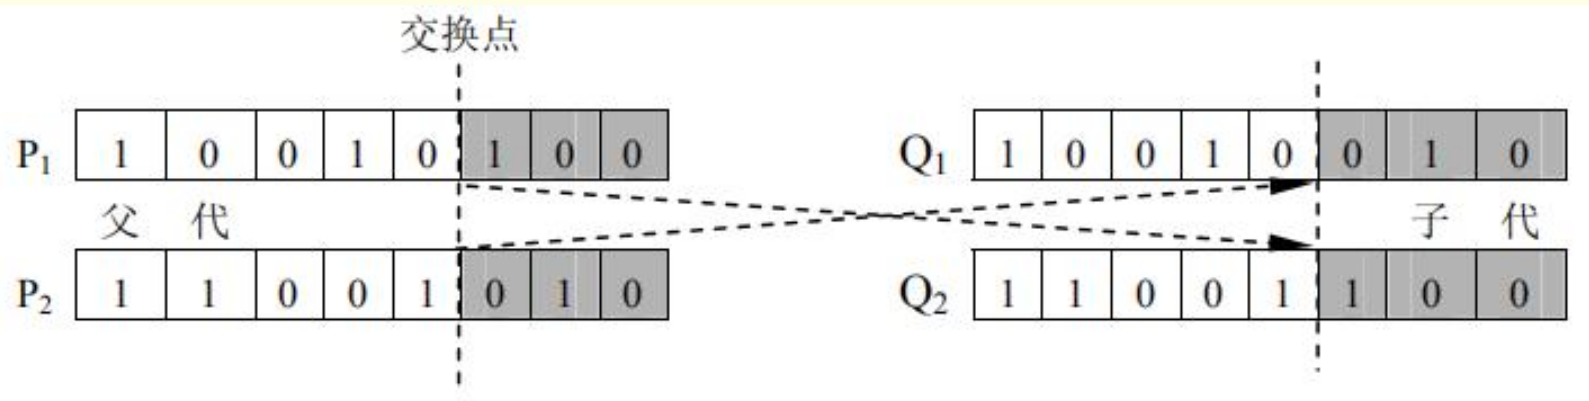
\includegraphics[scale=0.3]{/home/wty/Documents/LaTex-Projects/Nature Computation/simple_genetic_algorithm/简单遗传算法及例题求解.assets/交叉操作.png}
\caption{交叉操作}
\end{figure}

\begin{pythoncode}
idxs = np.random.choice(self.M, int(self.M * self.pc // 2 * 2))  # 选出交换个体下标
for i in range(int(self.M * self.pc // 2)):
    a, b = y[idxs[i<<1]], y[idxs[i<<1|1]]  # 抽取两个个体
    qc = np.random.randint(0, self.L) + 1  # 交换前qc位
    c, d = a.copy(), b.copy()  # 先保存在c,d上
    a = ((a >> qc) << qc) + (d & ((1<<qc) - 1))  # 交换
    b = ((b >> qc) << qc) + (c & ((1<<qc) - 1))  # 交换
    y[idxs[i<<1]], y[idxs[i<<1|1]] = a, b
\end{pythoncode}

\textbf{6. 变异操作}

设变异概率为
\(p_m\)(0.005\textasciitilde0.01),对于每个交叉后的个体,在 \([1,L]\)
上的每一位都有 \(p_m\)
的概率发生变异(0和1的互换,异或操作:\(0\gets1,1\gets0\)),给定变异概率
\(p_m\) 后,总共期望发生的变异位数为 \(B = M\cdot L\cdot p_m\);

种群规模为 \(M=3\),编码长度为 \(L=4\),变异概率为 \(p_m=0.005\)
的一次变异操作例子如下:

\begin{figure}[htbp]
\centering
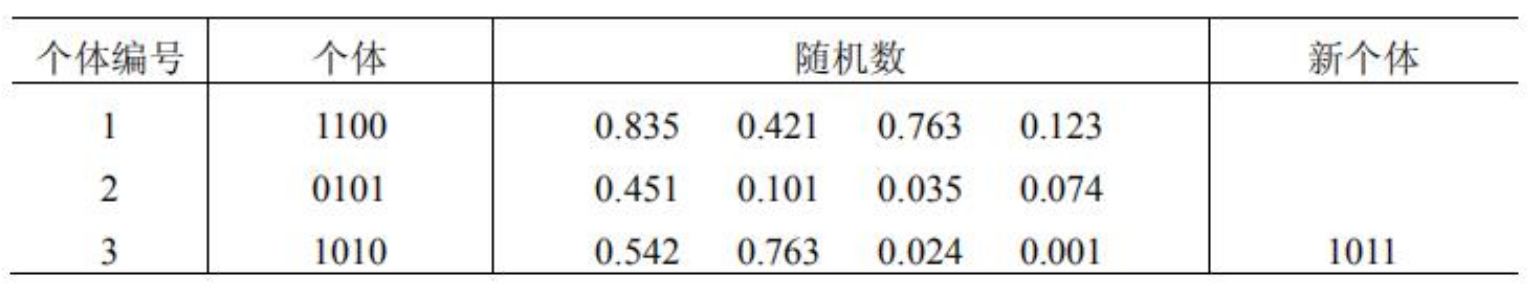
\includegraphics[scale=0.3]{/home/wty/Documents/LaTex-Projects/Nature Computation/simple_genetic_algorithm/简单遗传算法及例题求解.assets/变异操作.png}
\caption{变异操作}
\end{figure}
对每个个体的每一位生成一个 \([0,1)\) 之间的随机数 \(r\),如果
\(r \leqslant p_m\),则对该位置进行一次异或操作,例如个体编号为1,2的每一位的随机数都大于
\(0.005\) ,所以不进行变异操作;而编号为3的个体的第四位随机数
\(0.001 \leqslant 0.005\),所以只对第四位进行异或操作
\(0\gets 1\),于是变异结果为 \(1011\)。

\begin{pythoncode}
for i in range(len(y)):
    for j in range(self.L):  # 枚举y[i]的第j位
        if np.random.rand() <= self.pm:  # 如果发生变异
            y[i] ^= (1<<j)  # 对第j位进行异或    
\end{pythoncode}


\textbf{7. 终止条件}

执行上述步骤1,2之后,循环执行自然选择过程:3,4,5,6,直到达到终止条退出循环,终止条件常用有两种:

\begin{enumerate}
\def\labelenumi{\arabic{enumi}.}
\item
  最大迭代次数 \(N\)(200~500)
\item
  如果已知问题最优解 \(f^*\),则可设置终止条件为
  \(|f^{(i)}_{\max}-f^*|\leqslant \delta\)(其中 \(f^{(i)}_{\max}\) 表示
  \(1\sim i\) 次迭代中所有个体的最优适应度)
\end{enumerate}
\textbf{完整代码实现}:
\begin{pythoncode}
# -*- coding: utf-8 -*-
'''
@File    : sga.py
@Time    : 2023/04/28 11:29:27
@Author  : wty-yy
@Version : 1.0
@Blog    : https://wty-yy.space/
@Desc    : 简单遗传算法SGA在[-1,2]上最大化f(x)=x*sin(4*pi*x)+x**2,精确6位小数
'''
import numpy as np
import matplotlib.pyplot as plt
from scipy.optimize import differential_evolution  # 比较结果误差
from pathlib import Path
PATH_FIGURES = Path(__file__).parent  # 当前代码文件夹作为图片路径

def show_scipy_min():
    g = lambda x: -1 * f(x)
    res = differential_evolution(g, bounds=[(-1, 2)], tol=1e-6)
    print(f"scipy: 最优值 f({res.x[0]:.6f}) = {-res.fun:.6f}")
    return -res.fun

class SGA:
    def __init__(self, xmin, xmax, func, delta=1e-6, M=30, pc=0.8, pm=0.005, N=200):
        self.xmin, self.xmax, self.func, self.delta = xmin, xmax, func, delta
        self.M, self.pc, self.pm, self.N = M, pc, pm, N  # 超参数
        self.best = {'f': -np.inf, 'x': 0}
        self.logs = {'p_means': [], 'f_means': []}
        # 1. 计算编码长度L
        self.L = np.ceil(np.log2((self.xmax-self.xmin) / self.delta + 1)).astype(int)

    def decode(self, y):
        return self.xmin + (self.xmax - self.xmin) / ((1<<self.L) - 1) * y
    
    def solve(self):
        # 2. 随机产生初始群体
        y = np.random.randint(0, 1<<self.L, size=self.M)
        for _ in range(self.N):
            # 3. 计算适应度值(得分)
            s = self.func(self.decode(y))
            if np.max(s) > self.best['f']:
                self.best['f'] = np.max(s)
                self.best['x'] = self.decode(y[np.argmax(s)])
            self.logs['p_means'].append(np.mean(y))
            self.logs['f_means'].append(np.mean(s))
            # 4. 每个个体的选择概率(概率分布)加上1e-8是避免除0
            p = (s - s.min() + 1e-8) / np.sum(s - s.min() + 1e-8)
            y = y[np.random.choice(self.M, self.M, p=p)]
            # 5. 交叉操作
            idxs = np.random.choice(self.M, int(self.M * self.pc // 2 * 2))
            for i in range(int(self.M * self.pc // 2)):
                a, b = y[idxs[i<<1]], y[idxs[i<<1|1]]
                qc = np.random.randint(0, self.L) + 1  # 交换前qc位
                c, d = a.copy(), b.copy()
                a = ((a >> qc) << qc) + (d & ((1<<qc) - 1))
                b = ((b >> qc) << qc) + (c & ((1<<qc) - 1))
                y[idxs[i<<1]], y[idxs[i<<1|1]] = a, b
            # 6. 变异操作
            for i in range(len(y)):
                for j in range(self.L):
                    if np.random.rand() <= self.pm:
                        y[i] ^= (1<<j)
        print(f"SGA: 最优值 f({self.best['x']:.6f}) = {self.best['f']:.6f}")
        return self.best['f']

def f(x): return x * np.sin(4 * np.pi * x) + x ** 2

if __name__ == '__main__':
    sga = SGA(-1, 2, func=f)
    sga_best = sga.solve()
    true_best = show_scipy_min()
    print(f"误差: {np.abs(sga_best - true_best)}")
    
    logs = sga.logs
    fig, ax = plt.subplots(figsize=(8, 5))
    means = np.array(logs['p_means'])
    means = (means - means.min()) / (means.max() - means.min())
    ax.plot(logs['f_means'], '-*', label='f mean')
    ax.plot(means + 4.5, '-*', label='Population mean')
    ax.plot([0, 500], [4.300863, 4.300863], '--r', label='True best')
    ax.set_xlim(0, 25)
    ax.legend()
    fig.tight_layout()
    fig.savefig(PATH_FIGURES.joinpath("plot_sga.png"), dpi=300)
    plt.show()
\end{pythoncode}
\end{solution}

下面是一次程序的输出结果:

\begin{pythoncode}
SGA: 最优值 f(1.641580) = 4.300863
scipy: 最优值 f(1.641559) = 4.300863
误差: 5.509082079413474e-08
\end{pythoncode}

\begin{figure}[htbp]
\centering
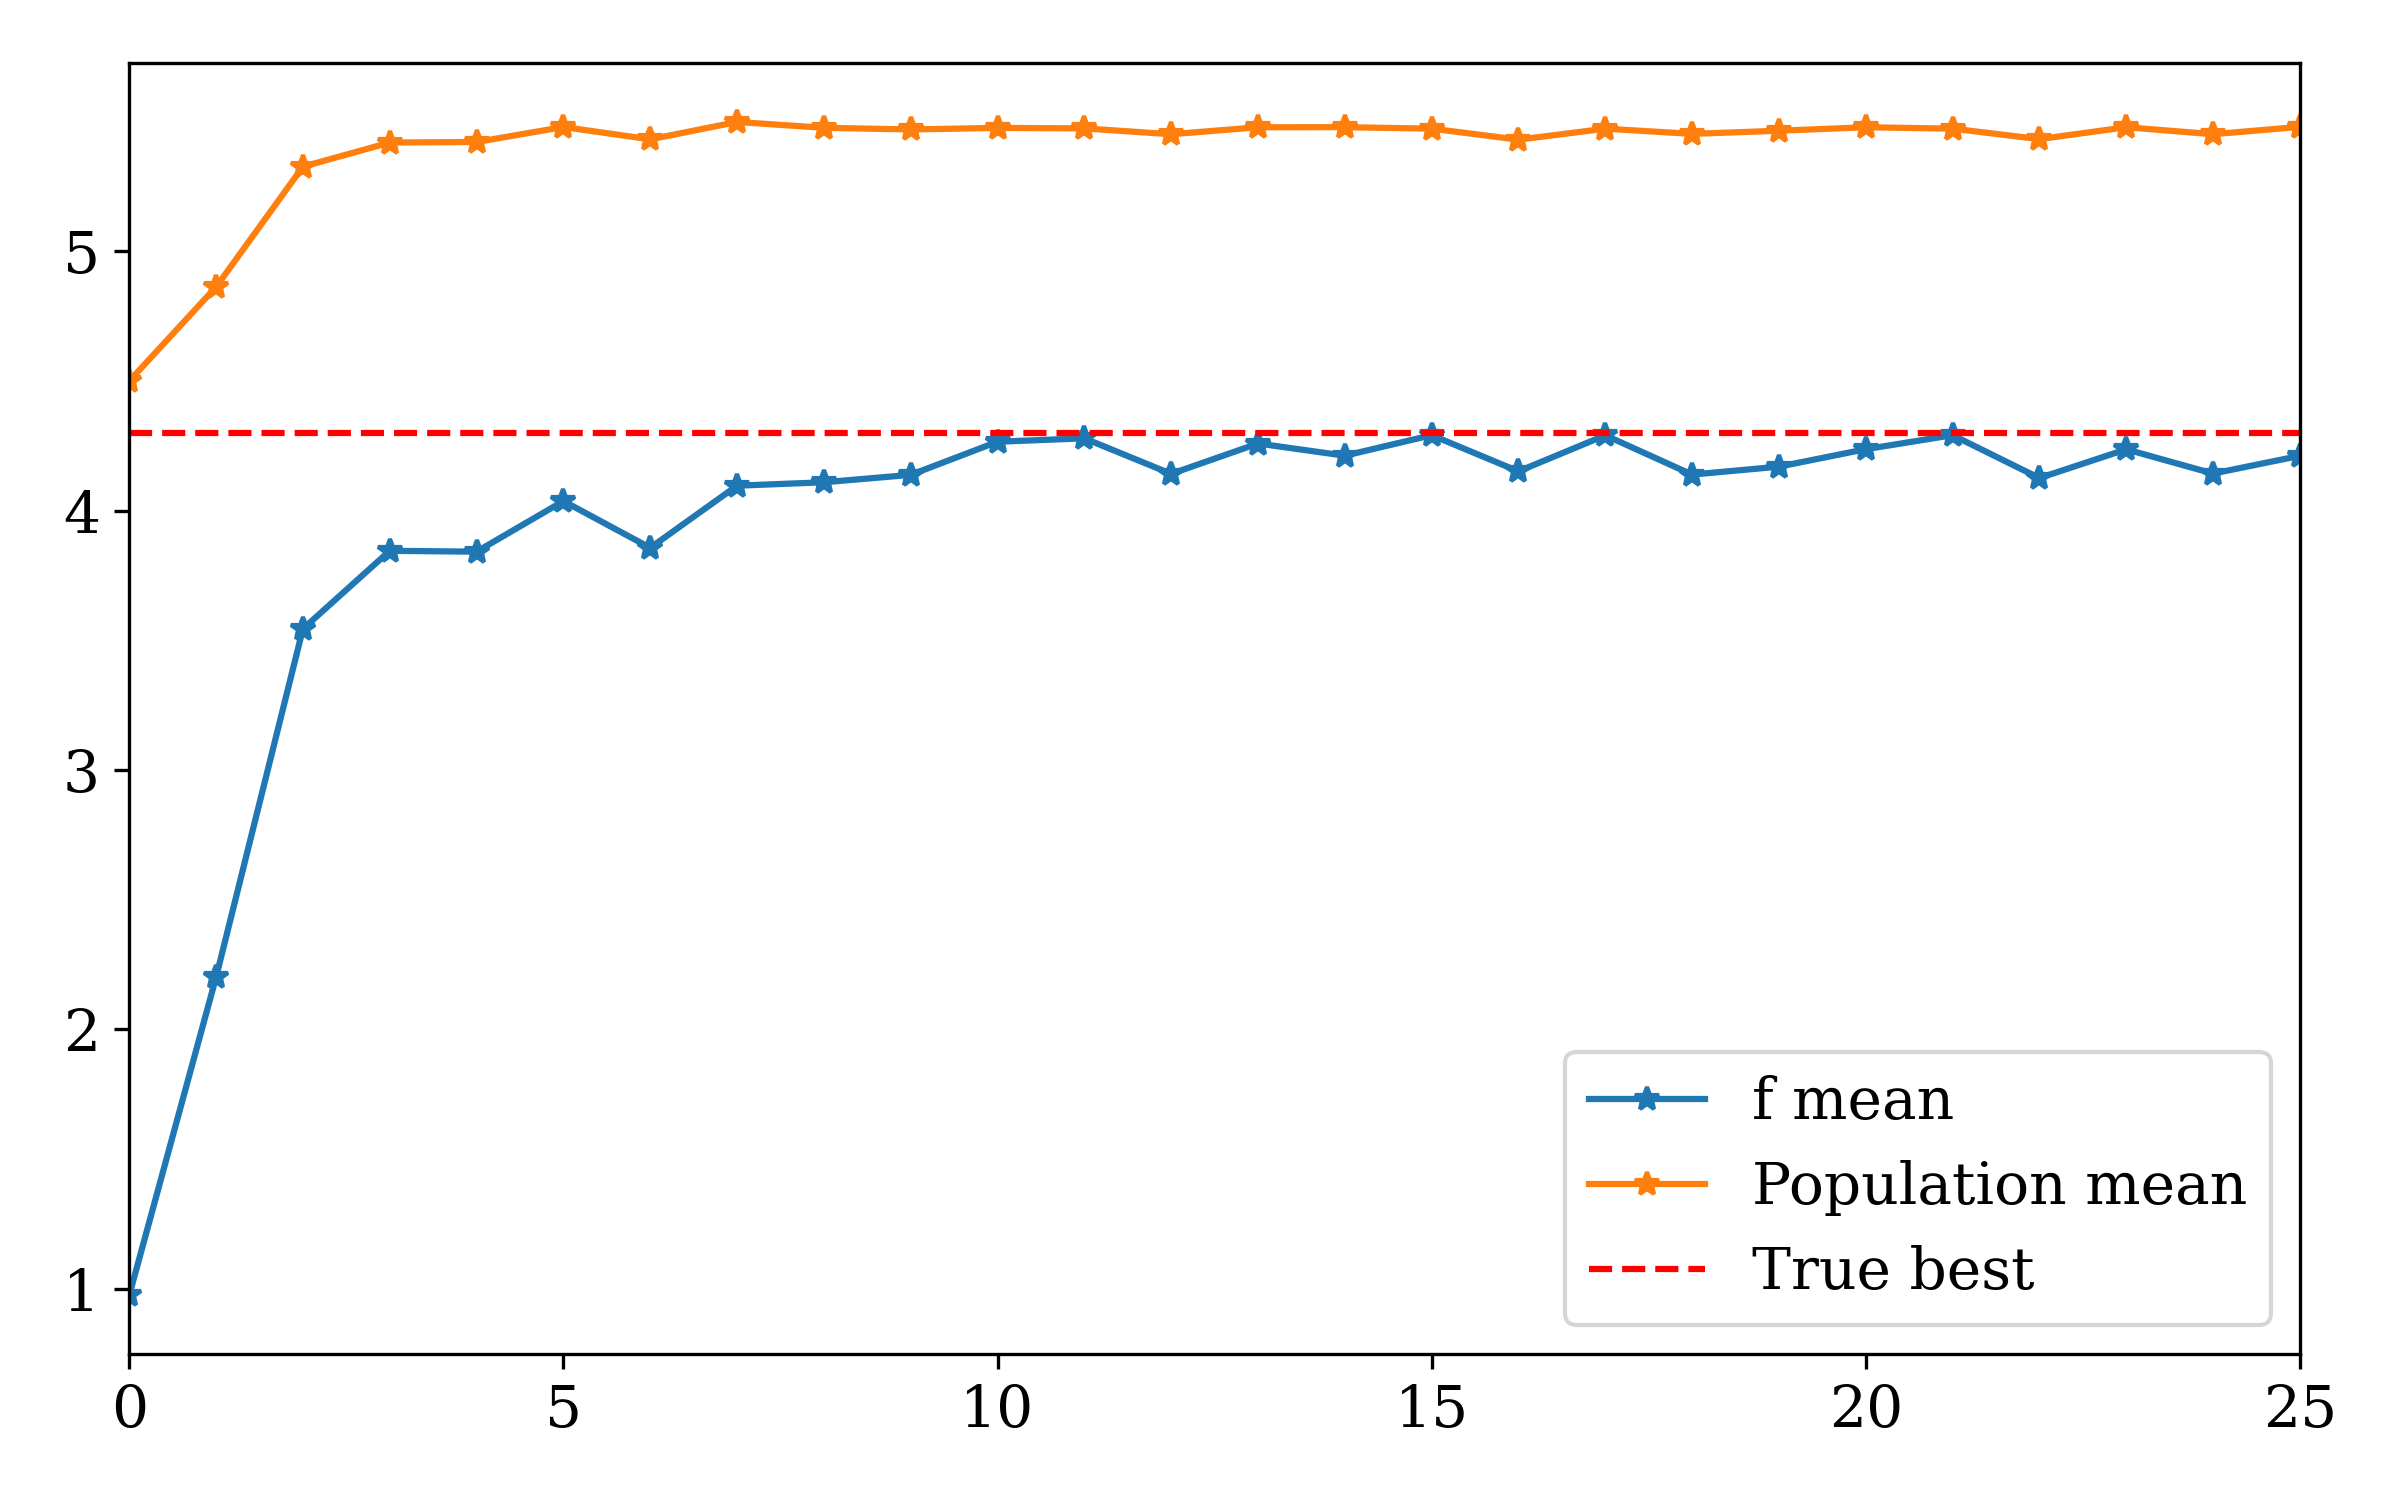
\includegraphics[scale=0.8]{/home/wty/Documents/LaTex-Projects/Nature Computation/simple_genetic_algorithm/简单遗传算法及例题求解.assets/plot_sga.png}
\caption{变换趋势图}
\end{figure}

我进一步对不同的超参数进行比较,得到下图4:(完整代码见我的\href{https://github.com/wty-yy/LaTex-Projects/tree/main/Nature%20Computation/code_SGA}{GitHub - code\_SGA})

不难发现种群大小$M$不宜太大$30$的效果就比$100$要好,可能是我取得是$f(x)$均值缘故;交叉率$p_c$值在最终状态基本一直相同,
只是在开始时$p_c=0.5$要更优;变异率$p_m$值有明显的区别,对于该问题,变异率为$0.005$效果更好,可能因为问题较为简单。

\begin{figure}[htbp]
\hspace{-0.5cm}
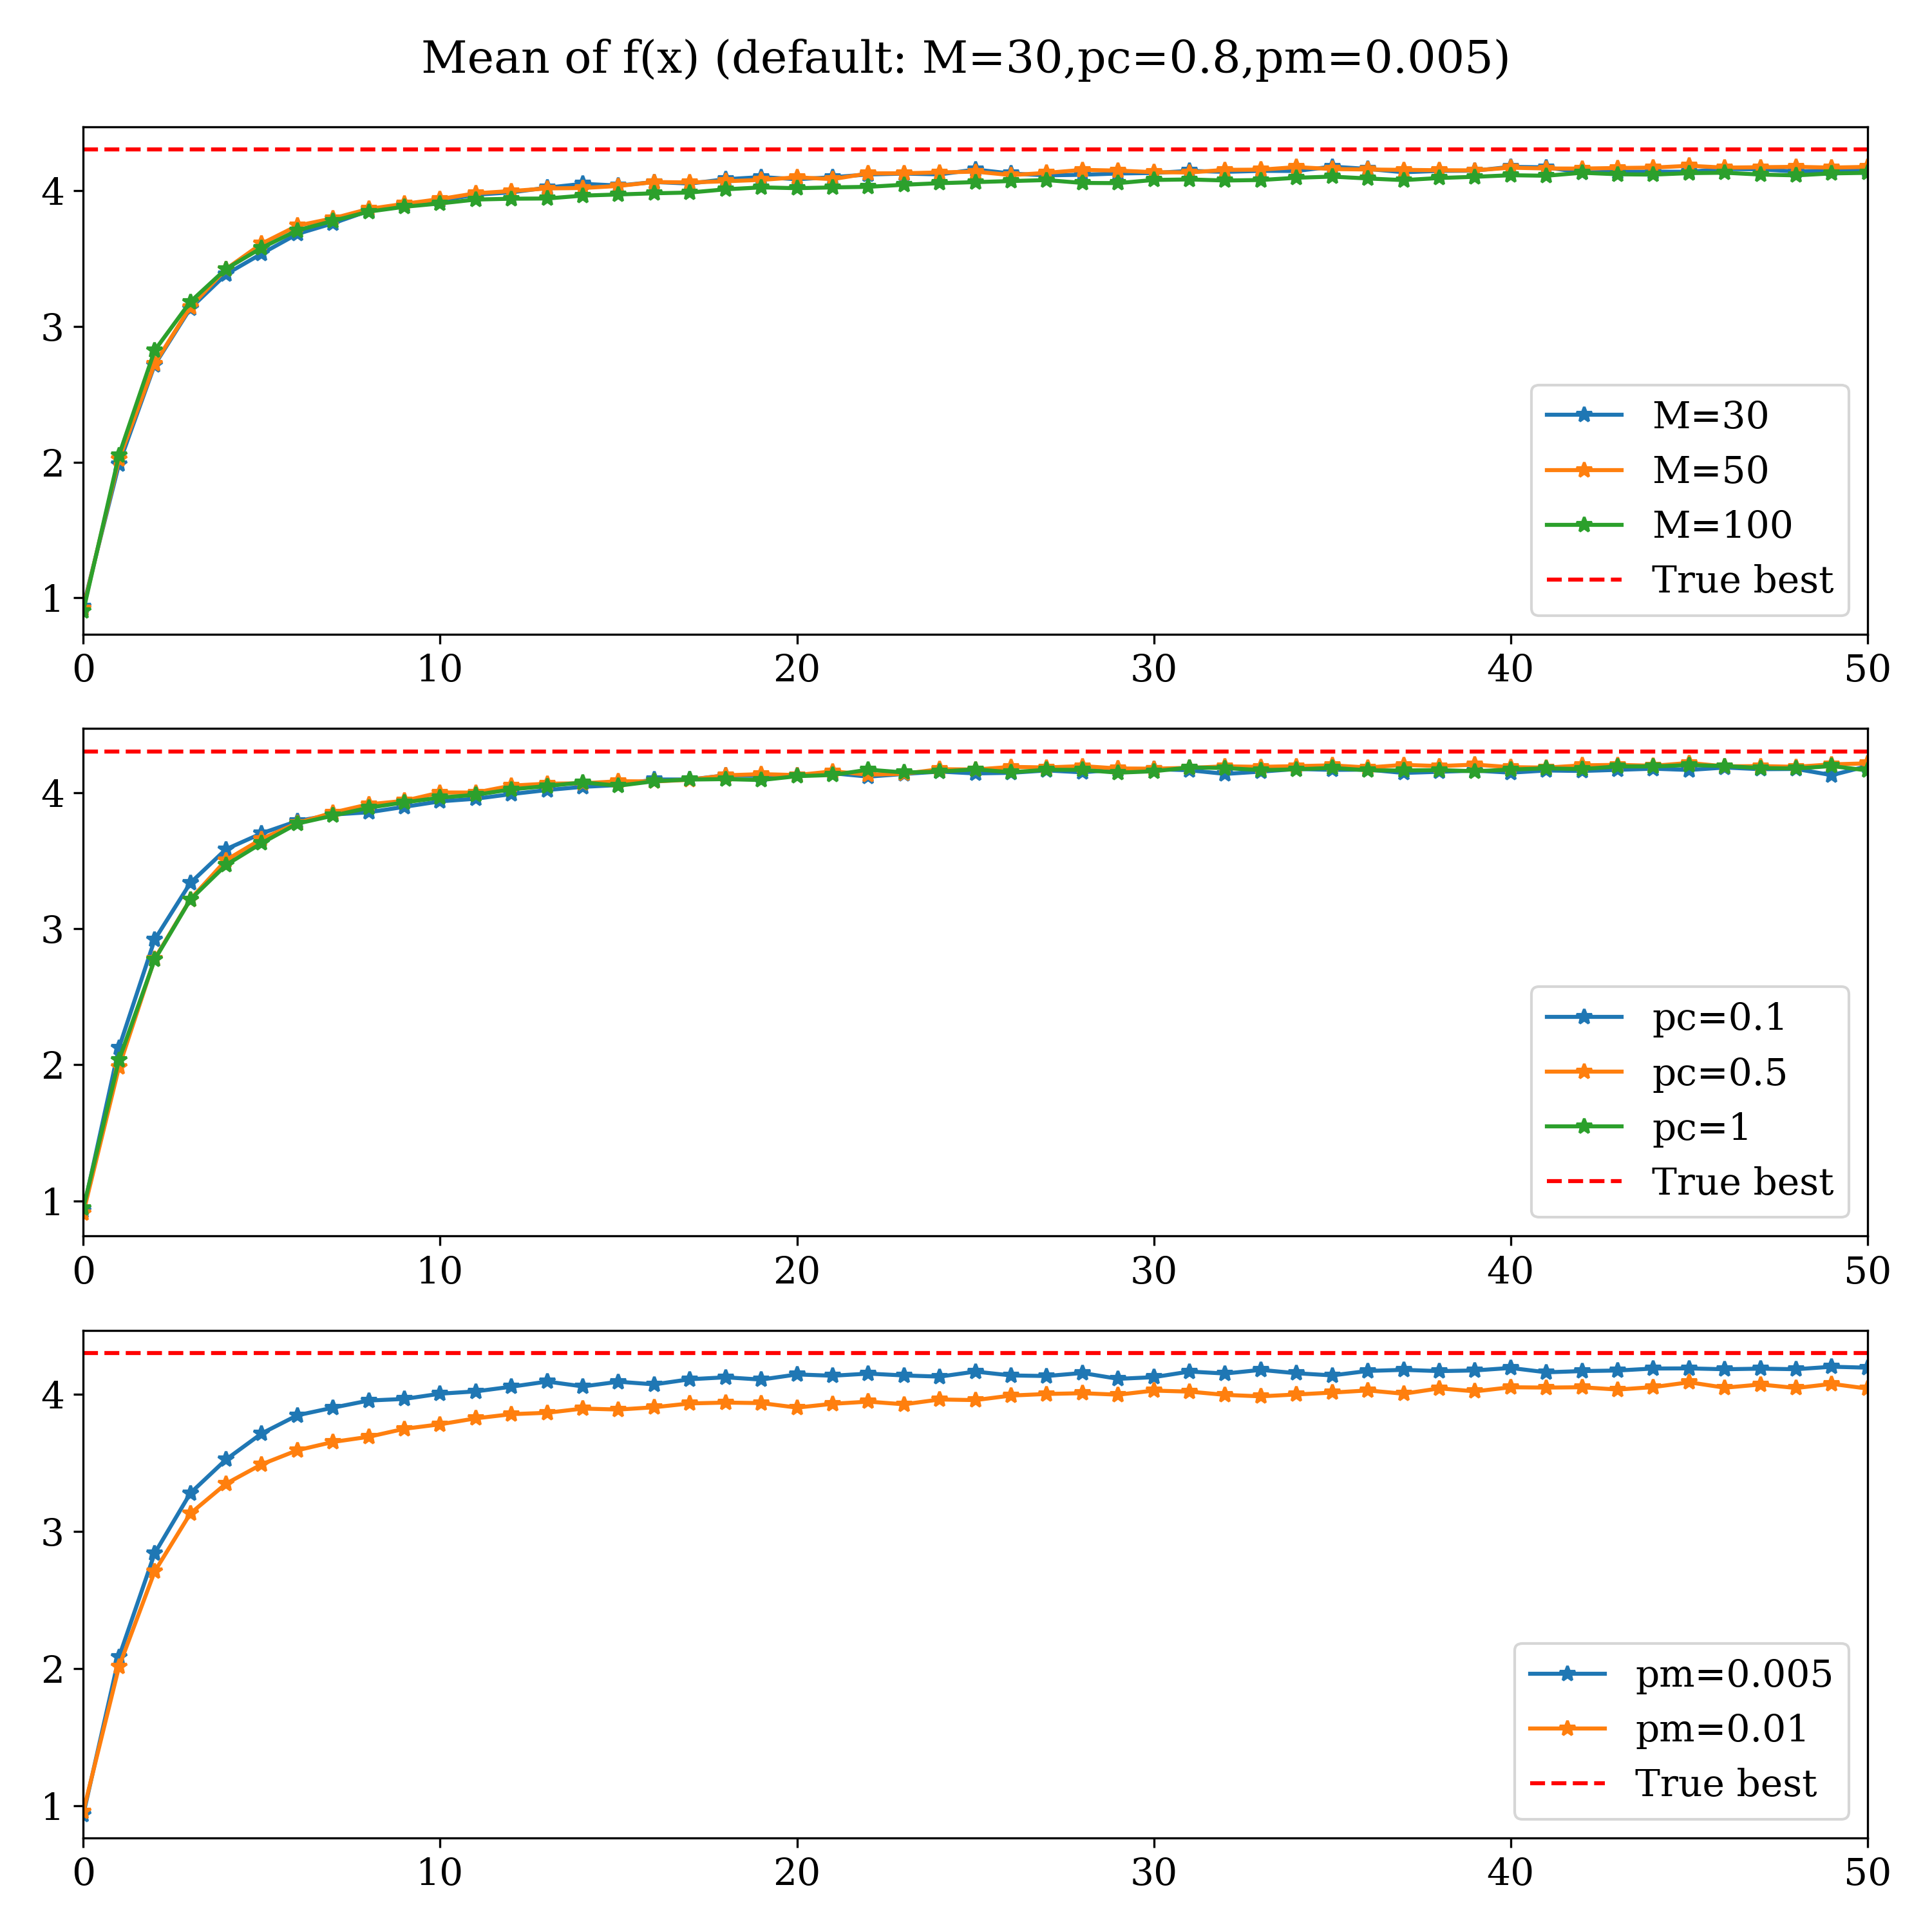
\includegraphics[scale=0.7]{/home/wty/Documents/LaTex-Projects/Nature Computation/simple_genetic_algorithm/简单遗传算法及例题求解.assets/parameter_compare.png}
\caption{不同超参数对比}
\end{figure}
\end{document}